\documentclass[a4paper,11pt]{scrartcl}

\newif{\iftth}

%\usepackage{latex2man}

\usepackage[utf8x]{inputenc}
\usepackage[T1]{fontenc}
\usepackage[american]{babel}
\usepackage{times}
\usepackage{listings}
\usepackage{graphicx}
\usepackage{wrapfig}
\usepackage{amsmath}
\usepackage{hyperref}


%\lstset{language=XML,stepnumber=1,basicstyle=\small}

\hypersetup{
pdftitle={Smrender – A rule-based Renderer for OSM Data},
pdfauthor={Bernhard R. Fischer, 2048R/5C5FFD47, <bf@abenteuerland.at>},
pdfsubject={},
pdfkeywords={renderer,sea map,sea chart,osm,openstreetmap,openseamap,xml,png,pdf,svg,kap,bsb,C,framework,data processing,scripting},
pdflang={en}
}

\newcommand{\optk}[1]{\textsf{\small\textbf{-#1}}}
\newcommand{\optv}[1]{\textsf{\small\underline{#1}}}
\newcommand{\opt}[2]{\optk{#1} $<$\optv{#2}$>$}

\newcommand{\rbox}[1]{\noindent\fbox{\texttt{#1\strut}}}

\newcommand{\smrender}{{\sffamily\slshape\small Smrender}}

\newcommand{\flinput}[1]{%
\iftth\verbatiminput{#1}%
\else\lstinputlisting[language=C,basicstyle=\footnotesize]{#1}%
\fi%
}

\title{Smrender -- A rule-based Renderer for OSM Data}
\author{Bernhard R. Fischer}


\setlength{\oddsidemargin}{27.5pt}
\setlength{\topmargin}{-34.6pt}
\setlength{\textwidth}{428pt}
\setlength{\textheight}{49\baselineskip}
\setlength{\parindent}{0pt}

%\renewcommand{\baselinestretch}{1.5}


\makeatletter
\def\thickhrulefill{\leavevmode \leaders \hrule height 1pt\hfill \kern \z@}
\renewcommand{\maketitle}{\begin{titlepage}%                               
    \let\footnotesize\small                                                
    \let\footnoterule\relax                                                
    \parindent \z@                                                         
    \reset@font                                                            
    \null                                                                  

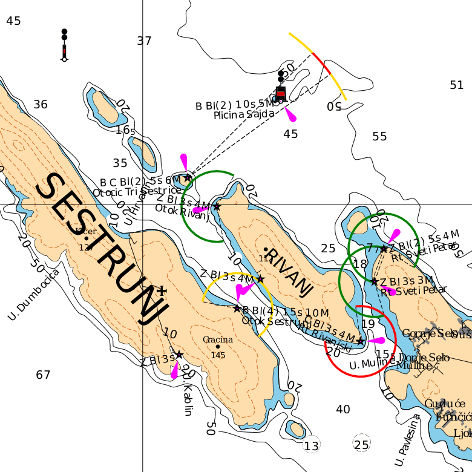
\includegraphics[]{inc/titlepic}
    \vskip 20\p@                      
\vfil                                 
    \hrule height 4pt                 
    \vskip 10\p@                      
    \begin{flushright}                
      \Huge                           
      \strut Smrender \par             
      \Large
\vskip 15\p@
      A Rule-based Renderer for OSM Data
%      Welchen Einfluss haben Massenmedien 
%
%      auf Familien im ländlichen Raum
%
%      im Mostviertel Niederösterreichs?
%
      \LARGE                          
      \vskip 30\p@                    
      \strut \@author
       \vskip 30\p@                   
\normalsize                           
      \strut \today
%\small                               
       \vskip 6\p@                    
%      \strut Theorie des wissenschaftlichen Arbeitens
    \end{flushright}                                                       
    \vskip 5\p@                                                            
    \hrule height 4pt                                                      
    \vskip 20\p@                                                           
    \vfil                                                                  
%\tableofcontents                                                           
%\centering                                                                
%\includegraphics[scale=.7]{pics/title}                                    
   \null                                                                   
  \end{titlepage}%                                                         
  \setcounter{footnote}{0}%                                                
}                                                                          

\makeatother




\begin{document}

\maketitle

\clearpage

\tableofcontents


\vfill 
{\raggedleft

\includegraphics[scale=0.5]{inc/schneggendier_600dpi_16mm}

}

\clearpage

\section{Release Notes}

This document describes the current (2015/08/22) version of \smrender{} which
is tagged as version 4.0. The document corresponds to the internal SVN revision number 1854
of \smrender{}. Starting with version 3.0 \smrender{} supports
\textsf{libcairo}\footnote{\url{http://www.cairographics.org/}} instead of
\textsf{libgd} as its graphical library.
There are some major changes after SVN revision 1240, thus this document
does not apply to revisions 1240 and earlier. The format of the ruleset changed
and are \textbf{not} compatible.

Unfortunately, this documentation is not complete yet, but I will continue to
work on it.

%The basic concept of \smrender{} will not change with future versions but there
%are several constructions which will probably change. This is most notably
%the format of the actions and their parameters. They just evolved at random
%during development without any structure. It will be changed to have a
%well-formed structure also that parts of the code will be rewritten, to be more
%than just a prototype.

\smrender{} contains several functions which are experimental. Those functions
are namely the auto-rotation and the polygon-size dependent captions (see
Section \ref{sec:cap}).

\section{Name}

\smrender{} is a universal rule-based rendering engine for OSM data. Because
\smrender{} is a very generic and flexible OSM processing engine, it may be used
for different tasks such as data filtering or data modification.

\section{Synopsis}

\noindent\textsf{\textbf{smrender} [OPTIONS]} [\optv{window}]

\section{Description} \label{sec:descr}

Smrender reads an OSM file and applies a set of rules to this input data to
create an output image. The input is an OSM file and a set of files containing
the rule set. Supported output formats are currently PDF, SVG, PNG, and KAP/BSB\footnote{\url{http://opencpn.org/ocpn/kap_format}}
having the desired resolution and density. Additionally, some other output
files may be generated depending in the rule set. The latter is explained
later.

The primary goal of \smrender{} is to create a sea chart which is well-suited for
print-out on paper. Nevertheless, it is a universal rendering engine and may be
used for different tasks.

The input file should be an OSM/XML file as defined by the OSM standard. The
file is required to be well-formed in that sense because \smrender{} itself does
no XML validation, thus the rendering process might fail if the file is not
well-formed.  The data should also be complete. This means that it should
contain all nodes to which is referred by the ways. \smrender{} will remove nodes
from ways which are missing.

The rules are also defined in OSM format (see Section \ref{sec:rules}). The
rules are applied iteratively in a loop depending on their \emph{version}.
Within the loop, \smrender{} always applies first all relation rules, then way rules, and then all node
rules of the same version. All rules of the same version are applied in the
order of their \emph{id}.

Invisible objects are ignored by the renderer. Invisible objects are such which
have set the attribute \textsf{visible=``false''}.  If objects have no such
attribute \smrender{} sets it to ``true'' by default.

\subsection{Rendering Window} \label{sec:window}

Smrender renders an area which is specified by the \optv{window}. It is a compound
argument as defined below.
\begin{verbatim}
   <window>      := <center> | <bbox>
   <bbox>        := <left lower>:<right upper>
   <left lower>  := <coords>
   <right upper> := <coords>
   <center>      := <coords> ':' <size>
   <coords>      := <dec_coords> | <naut_coords>
   <dec_coords>  := <lat> ':' <lon>
   <naut_coords> := ( <naut_lat> ':' <naut_lon ) | 
                    ( <naut_lon> ':' <naut_lat> )
   <size>        := <scale> | <length> 'd' | <length> 'm'
\end{verbatim}
The area to be rendered is either specified by a center point of the
area or a bounding box.

If it is chosen to use a center point specification then
\optv{lat} and \optv{lon} set the center coordinates in latitude and longitude
in degrees in WGS84 reference system. Although it can be any valid
coordinate, it is suggested to choose an ``even'' value rounded to 10 minutes
(e.g. 43.666667 which is 43° 40').

Alternatively, the coordinates can be given in nautical notation which is
\textsf{dd C mm.m} where \textsf{dd} is degrees as integer value, \textsf{C} is one of
'N', 'S', 'E', or 'W', and \textsf{mm.m} are minutes, for example
\textsf{43N40}. In case of nautical notation, \smrender{} automatically detects
which of the the values is the latitude and which is the longitude dependent on
the character used for the cardinal direction.

\optv{Length} defines the length of the mean latitude (parallel) in degrees if
\textsf{'d'} is appended or in nautical miles if \textsf{'m'} is appended.
Alternatively, the \optv{scale} of the chart can be specified. \smrender{}
calculates the size of the area to meet the scale. Obviously, this depends on the size
of the output image. The height (the length of the mean longitude) is
calculated automatically by \smrender{} in such a way that the output image is
projected correctly using a \emph{Mercartor projection}. The height depends on the size
of the output image (page format).\\

If it is chosen to use a bounding box specification then the coordinates of the
left lower (southern western) and the right upper (northern eastern) point
shall be specified. Because of the projection the bounding box must not
necessarily fit to the page dimension in which case \smrender{} will
automatically resize the bounding box to fit to the page.  If a fixed bounding
box is desired the option \optk{P} is needed with either the width or the
height set to zero. In this case \smrender{} will calculate a page dimension
which fits to the bounding box according to the projection.\\

If this argument is omitted The value 0:0:100000 is chosen as default and the
option \optk{a} is set implicitly.

\subsection{Options} \label{sec:options}

\begin{itemize}

%\item[\optk{C}]
%   Do not close open coastline polylines.
%
%   For the renderer to be able to fill the land areas (continents,
%   islands,\ldots) with a specific color, those polygons must be closed. In OSM
%   the coastline typically is not one large closed polygon but rather a set of
%   shorter polylines. The adjacent ones share the same start/end nodes.
%   Furthermore just a specific region (the \emph{bounding box}) is
%   selected for rendering and not the whole planet. Obviously, the coastline of
%   large islands or the continents stay open on the border of the selection.
%
%   This option suppresses the closing process. This option is useful if
%   smrender should be used in \emph{filter mode} (see Section
%   \ref{sec:filter}).

   \item[\optk{a}]

      \smrender{} usually processes just those nodes which are located within
      the window of rendering (see Section \ref{sec:window}). This behavior is new with
      version 3.0.  With this option set \smrender{} processes all nodes
      independently of their location.

   \item[\optk{b}] \optv{color}

      This option allows to set a background color. The color may be define either as a color preset
      or an HTML-style definition (see Section \ref{sec:cap}). The default color is white.

      Please note that some Shells (such as the \textsf{bash}) interpret the
      \textsf{\#} character if the color is specified in HTML-style. In this
      case you have to put the color specification under single or double quotes, e.g. \textsf{-b '\#8080ff'}.

   \item [\optk{D}] 

      \smrender{} outputs a lot of information to stderr to watch the progress of
      rendering. It uses the same log levels as defined for syslog (see
      \textsf{syslog(3)}). By default it logs all messages of the log level
      \textsf{LOG\_INFO} and above. With this option also debug messages are
      printed. This may be useful if something goes wrong.

\item[\optk{d}] \optv{density} %\opt{d}{density}
   
   Set the \optv{density} of the output image. The default value is 300 which
   is typically used for print-outs in good quality. This option does only
   apply if you produce pixel (raster) images such as PNG or JPG.

\item[\optk{f}]

   Filter data while loading the input file.

   With this option a bounding box is used to load just those nodes and ways
   which are within the selection.  The bounding box is 10\% larger then the
   area which resumes from the selected \optv{window}.
   This option is useful if huge input data sets are used, such as the planet
   file.

   Please note that this option works only correctly if the nodes and ways are
   stored in that order in the input file (first all nodes and then all
   ways).

\item[\optk{g}] \optv{d}[:\optv{t}[:\optv{s}{]}{]}

   This option defines the distance \optv{d} of the grid lines in minutes. The
   border of the chart (latitude and longitude axis) also depends on this
   setting. As it is usual for sea charts, there is a major and a minor axis
   scale, called ticks and subticks. The ticks are defined by \optv{t} and the subticks
   are defined by \optv{s} in minutes. For a correct result, \optv{t} as well
   as \optv{d} should be integral multiples of \optv{s}.

   Note that \smrender{} internally uses a precision of hundreds of a minute while doing
   the grid calculation. Thus, the smallest granularity for the grid parameters is 0.01 minutes.

   If this option is omitted, \smrender{} will choose a grid setting dependent
   on the scale of the output image. For scales below 1:150000 it chooses
   5:1:0.2, for scales below 1:250000 it chooses 10:1:0.25, and for scales
   above 1:250000 it is set to 20:2:0.5.

   A grid may optionally be generated with the action \textsf{grid}. See
   Section \ref{sec:special}.
   
\item[\optk{G}]

   Do not generate grid nodes/ways. \smrender{} actually does not render the grid directly onto the output
   image but rather generates regular OSM nodes and ways. These objects are then rendered in a way as
   it is defined by the regular rule set.
   All ways of the grid are tagged with \textsf{grid=*}. Part of the grid are also labels on the border
   showing degrees in latitude an longitude. The labels are nodes which are tagged with \textsf{grid=text}
   and the tag \textsf{name=*} containing the value.

\item[\optk{h}]

   Output the list of available options and a short description to stdout and
   exit.

\item[\optk{i}] \optv{file}

   This option specifies the name of the input \optv{file}. If this option is omitted, \smrender{} reads
   from \textsf{stdin}.

\item[\optk{k}] \optv{file}

   With this option \smrender{} will write a KAP/BSB file to \optv{file}
   which can be used with most navigation applications and GPS devices.  See Section \ref{sec:genkap} for
   more details.

\item[\optk{K}] \optv{file}

   This is similar to option \optk{k} but it generates only a KAP/BSB header
   instead of a complete file. This is useful if you want to use an external
   tool such as \textsf{imgkap} to create the KAP file from the PNG.

\item[\optk{l}]

   Output page has landscape format rather than portrait, which is default. This option is used only in conjunction
   with option \optk{P} if a literal page format is used.

\item[\optk{o}] \optv{file}

   Set the filename of the output image. \smrender{} parses the string and
   chooses the output file dependent on the file extensions which can be one of
   \textsf{.pdf}, \textsf{.png}, or \textsf{.svg}. It defaults to PNG if no
   valid extension was found.
   If this option is omitted no image file will be generated.

\item[\optk{O}] \optv{file}

   Create output PDF file. This option is \emph{deprecated}. See option \optk{o}.

\item[\optk{P}] \optv{fmt\textbar geom}

   Select the page format of the output image. The format can be set either named format \optv{fmt} which
   has a specific dimension or as geometry \optv{geom} which contains the width and height of the page
   in millimeters in the format \optv{width}\textsf{x}\optv{height}.
   \optv{Fmt} currently supports the values \textsf{A4} up to \textsf{A0}.
   If this option is omitted, \textsf{A3} format is selected by default.

   If the area to be rendered is specified as bounding box (see Section
   \ref{sec:window}) this will most probably colide with the dimension of the
   page because of the requirements of the projection in which case \smrender{}
   will resize the bounding box appropriately. If either the \optv{width} or
   the \optv{height} (but never both) is set to zero then \smrender{} will
   calculate the missing dimension according to the bounding box and the
   projection.

\item[\optk{m}] Disable memory mapping (see option \optk{M}).

\item[\optk{M}]

   This option is mandatory if the input file is larger than the amount of memory available on the rendering system.
   If the system has enough memory this option can be omitted. Using memory mapping probably is a little
   bit slower but heavily depends on the operating system. On Linux kernel 2.6.32 there is no significant
   difference in speed.
   
   In any case, files which are larger then 2 GBytes are only supported on 64 bit operating systems.

   This option is now on by default.

\item[\optk{N}] \optv{ofs}
   
   With this option \smrender{} adds \optv{ofs} to all
   nodes and ways IDs as well as to the node references of the ways for all OSM
   files that are generated by \smrender{} by using the option \optk{w} or the
   action \textsf{out()} (see Section \ref{sec:output}).

   This options is mainly intended to renumber IDs from input files.

\item[\optk{n}] Some actions of \smrender{} generate new objects. Negative ids
   are added to those objects. If this data created by \smrender{} is fed to
   another OSM tool negative ids may cause problems. With this option all
   negative ids are output as positive values.

\item[\optk{r}] \optv{file}

   This option specifies the \optv{file} name of the rules file. If it is
   omitted, \smrender{} expects the rules file to be named \textsf{rules.osm}.
   If \optv{file} is set to \textsf{none} \smrender{} is run without rules.

   If \optv{file} is a directory \smrender{} will scan it and read all files
   which match ``\textsf{*osm}''.  The files are read in alphabetical order,
   simply compared with \textsf{strcmp(3)}. Thus, it is suggested to create
   symbolic links to the files in name it in an appropriate way similar to SysV
   init scripts.

   If you need a more specific order of rule execution you should consider to
   use the \textsf{version} and/or \textsf{id} fields of the OSM objects (see
   Section \ref{sec:descr}).

\item[\optk{R}] \optv{file}

   This option may be used to save the rules again to another OSM file. This fill will be well-formed in terms of OSM/XML
   format and may be loaded into JOSM.

\item[\optk{s}] \optv{f}

   This option scales all images used in the \textsf{img()} function by the
   factor \optv{f} (see Section \ref{sec:img}). By default this is 1. This
   factor is applied additionally to a scaling defined in \textsf{img()}.

\item[\optk{t}] \optv{title}

   This option generates a descriptional title node which can be rendered onto the
   final chart. It is as well used as a title for KAP files (see option \optk{k}).

\item[\optk{T}] \optv{z} ':' \optv{dir} [ ':' \optv{ftype} ]

   Create tiles suitable for an online viewer into the directory \optv{dir}.
   The zoom levels are specified by \optv{z} which can be either a single value
   or a range, e.g. 10-15.
   
   The optional parameter \optv{ftype} sets the file type of the tile images
   which can be either \textsf{png} (which is default) or \textsf{jpg}.

\item[\optk{u}]

   With this option \smrender{} will output a set of URLs which are suitable for
   OSM data download for the area of rendering specified by the \optv{window}.

\item[\optk{V}]

   With this option set, \smrender{} parses all arguments, and calculates and
   prints the rendering parameters to stderr. Then it exits immediately.

\item[\optk{v}]

   With this option \smrender{} will output the version information of
   \smrender{} and \textsf{libcairo} to stdout and exit immediately.

\item[\optk{w}] \optv{file}

   This option specifies the file name of an output OSM file. \smrender{} will dump all nodes/ways to this file that have been
   selected by the import process and all nodes/ways which have been generated during the rendering process.

   These nodes/ways include the objects generated for the grid and also the close coastline ways.
   Thus the output depends on the options \optk{f}, \optk{C}, and \optk{G}.

   If this option is omitted, no output will be generated.

\end{itemize}


\section{Ruleset Definition} \label{sec:rules}

The rule set is also defined in OSM format. It contains nodes, ways, and relations together
with tags. Nodes are considered to be rules for rendering nodes and ways are
rules applied to ways. Each object (node,  way, or relation) has a list of tags. These
tags represent patterns which are matched against the tags of the objects which
are to be rendered. The values of a tag's key (\textsf{k=``\ldots''}) and/or value
(\textsf{v=``\ldots''}) may be either just a string which is directly matched in a
case-sensitive manner or a special match operation (see Section \ref{sec:match}).
The match operations can be used for the key as well as for the value.

Each object has to have a special tag which defines the action that should
be carried out in case of a match. This tag has the form \textsf{\_action\_=*}. The actions are described
below in Section \ref{sec:act}.

The match algorithm always applies all tags to match, and all of them have to match in order
to execute the action. If just a single tag does not match, the node is skipped.


\subsection{Order of Rule Execution} \label{ref:ruleorder}

A typical ruleset consists of a set of node, way, and relation rules. It is
important to understand the order in which the rules are executed. Since a page
is flat and 2-dimensional, rules which are executed later may paint over those
that have been executed before.

As defined by the OSM
specification\footnote{\url{http://wiki.openstreetmap.org/wiki/Elements}} all
object types (nodes, ways, relations, also called \emph{elements}) have common
attributes. Beside the object type, \smrender{} uses the attributes
\textsf{version} and \textsf{id} to determine the order of rule execution. All
rules of the same version are rendered in the order of their id ascendingly
within each type of object. This is repeated for each version ascendingly until
the last rule (highest version and highes id). The following enumeration
outlines the rendering order.

\begin{enumerate}
   \item All objects are selected according to their version number, lowest
      number first.

   \item All objects with the same version number are selected according to
      their type: all relations before ways before nodes.

   \item All objects of the same type (and version) are chosen according to
      their id, lowest id first.
\end{enumerate}

Rules with a version greater or equal to $2^{16} = 0\text{x}10000 = 65536$ are
ignored.  The number of iterations, i.e. the number of different versions is
limited to \textsf{MAX\_ITER}\footnote{It is currently (21$^{st}$ of October
2014) defined to 64.} which is defined in \textsf{rdata.h}. Run \smrender{}
with option \optk{V} to see its value.

If the \textsf{version} attribute is missing it is set to 1 by default. All
objects without \textsf{id} are numbered ascendingly in the order in which they
occur in the rules file starting with some low negative value.

The attribute \textsf{visible} can be set to either \textsf{true} (which is
default if omitted) or \textsf{false}. Rules which are ``invisible'' are not
executed. This can be used to enable or disable a rule by default and can
further be used for conditional rendering (see \textsf{enable\_rule} in Section
\ref{sec:special}).

\subsection{Match Operations} \label{sec:match}

Basically there are the four different match operations \emph{string compare},
\emph{regular expression match}, \emph{greater than}, and \emph{less than}.
Additionally, all of them may be \emph{inverted}, or \emph{excluded}.\\

\begin{itemize}

\item
\emph{String compare} is the most basic match operation. It does an exact case-sensitive string compare.
The following tag matches all objects
which own the tag \textsf{seamark:light\_character=*}.

\rbox{<tag k='seamark:light\_character' v='{}'/>}

The empty value \textsf{v='{}'} represents a wildcard match. It matches any string.\\

\item 
\emph{Regular expressions} are invoked by enclosing the expression within two slashes \textsf{/\ldots/}
as it is usual in Perl and several other languages. The expression is interpreted as a POSIX extended regular expression (see manpages
\textsf{regex(3)} and \textsf{regex(7)}). The following expression matches any object
which is tagged with either \textsf{highway=primary} or \textsf{highway=secondary}.


\rbox{<tag k='highway' v='/\^{}(secondary$\vert$primary)\$/'/>}\\

\item
\smrender{} can interpret tag values as numerical values. Thus, it can do arithmetical comparisons
which is \emph{less than} ($<$) and \emph{greater than} ($>$).

The rule has to contain a number enclosed in square brackets. The direction of the brackets denotes the
comparison operation; $[x]$ means that the value of the tag should be lower than $x$ and $]x[$
matches if the tag value is greater than $x$. The tag value as well as $x$ are always
interpreted as decimal number with \textsf{double} precision.

Square brackets are used deliberately instead of angle brackets to avoid possible conflicts with
the XML format or buggy parsers.

The following rule matches all objects whose \textsf{seamark:light:range}-value is greater than 7.5.

\rbox{<tag k='seamark:light:range' v=']7.5['/>}

\item
   Match inversion is done by enclosing the match expression within exclamation marks.
   This inverts the match if and only if the expression without inversion would match. This means that if a tag would match
   the expression, the inversion would return ``false'' (no match). But it would not return
   ``true'' (match) if the expression would not match.

   The following expression would match all objects which have a tag with the key \textsf{seamark:type}
   but its value is neither \textsf{landmark} nor \textsf{light\_major}.

   \rbox{<tag k='seamark:type' v='!/landmark$\vert$light\_major/!'/>}

\item 
   Match exclusion is denoted by enclosing the match expression within tildes. It does not match objects
   with certain tags, i.e. it matches the absence of the given tag.  The
   following rule avoids matching of objects which have a tag
   \textsf{seamark=*}, i.e. all objects match which do not have such a
   \textsf{seamark=*} tag.

   \rbox{<tag k='\~{}seamark\~{}' v='{}'/>}

   \end{itemize}

\subsection{Rule Actions}
\label{sec:act}

\smrender{} supports a number of powerful built-in actions which are carried out upon
successful match. As already mentioned at the beginning of this Section,
actions are defined simply with the tag \textsf{\_action\_=*}. The actions are
actually function calls either within the code of \smrender{} or externally from a
dynamic library. Thus, there is an unlimited range of extensibility of
\smrender. A number of parameters may optionally be passed to the function. The order
of the parameters does not matter.

The following example shows an action which places an image at the position of
a node.\\

\rbox{<tag k='\_action\_' v='img:file=icons/Light\_Minor.png'/>}\\

The basic format of an action and basic values and types are defined as follows.

\begin{verbatim}
   <action> := <ref> [ ':' <param> [ ';' <param> [ ... ] ] ]
   <ref>    := <func> [ '@' <library> ]
   <param>  := <tparam> | <bparam>
   <tparam> := [ SEP ] <name> [ SEP ] '=' [ SEP ] <value> [ SEP ]
   <bparam> := [ SEP ] <name> [ SEP ] '=' [ SEP ] <bool> [ SEP ]
   <bool>   := 'yes' | 'no' | 'true' | 'false' | <num>
   <num>    := any decimal number
   SEP      := '`' | '"'
   <length> := <num> [ <udef> ]
   <udef>   := <pageunit> | <nautunit>
   <pageunit> := 'mm' | 'cm' | 'in' | 'px' | 'pt' | '"'
   <nautunit> := 'degrees' | 'deg' | 'min' | 
                 'm' | 'km' | 'ft' | 'nm' | 'sm'
\end{verbatim}

Every action consists of a symbol name \optv{ref} which is used to find the
appropriate function in \smrender or in a shared object\footnote{Function
   libraries, on Unix-based systems \textsf{.so} files, on Mac OSX
   \textsf{.dylib} files, and on Windows \textsf{.dll} files.}
and an optional set of
parameters. These are attribute/value pairs. The names of the attributes are
case-sensitive. A special \emph{type} exists which is the boolean type. It can
be set to the case-insensitive strings 'yes', 'no', 'true', or 'false', or to
any decimal number. 0 is interpreted as false all other values are considered
to be \emph{true}.

\smrender{} is shipped with a set of functions for rendering. Those are
capable to place captions (Section \ref{sec:cap}), drawing and filling (Section
\ref{sec:draw}), placing icons (Section \ref{sec:img}), generating OSM files
(Section \ref{sec:output}), do some special purpose operations (Section
\ref{sec:special}), and calling external library functions (Section
\ref{sec:func}). The latter is thought to be a simple but powerful interface
for third-party modules.

All functions are described in Section \ref{sec:renderfunc}.


\subsection{Measurement Units} \label{sec:units}

Starting with revision 1851 \smrender{} knows about a set of standard
measurement units.\footnote{Please note that not all functions already know
about that.} There are two groups of units. The first one is related to the
page to which the chart is rendered and the second group is related to
reallity. Units referred to the page are listed in Table \ref{fig:pageunits}
and those referred to reallity are shown in Table \ref{fig:realunits}.

Units are used in combination with a decimal value. As usual, the unit symbols
are written behind the number and may be separated with zero or more white
spaces.

\begin{table}[h]
   \centering
\begin{tabular}{c|l|l}
   Symbol(s) & Descripton & Conversion factor\\\hline
   \textsf{mm} & Millimeters & = 0.03937" = 0.3527 pt\\
   \textsf{cm} & Centimeters & = 10 mm\\
   \textsf{in} or " & Inches & = 25.4 mm = 72 pt = 300 px \\
   \textsf{px} & Pixel & = 0.0846 mm = 0,0033" (see below)\\
   \textsf{pt} & Points & =$\frac{1}{72}$"\\
\end{tabular}

\caption{Measurement units referred to the output page.}
\label{fig:pageunits}
\end{table}

Pixels do not have a fixed conversion factor. It depends on the pixel density
and it is \emph{only} important for raster image output. The density (dpi, dots
per inch) is set with the command line option \optk{d}. The default value is
300.

Please note that \smrender{} internally operates vector-based and the suggested
output format is PDF which is created as vector image as well. There are no pixels.

\begin{table}[h]
   \centering
\begin{tabular}{c|l|l}
   Symbol(s) & Descripton & Conversion factor\\\hline
   \textsf{nm} & Nautical miles & = 1852 m = 6076.12 ft \\
   \textsf{kbl} & Cable length & = 185.2 m = 0.1 nm\\
   \textsf{'} or \textsf{min} & Minutes & = 1 nm\\
   \textsf{°} or \textsf{deg} & Degrees & = 60'\\
   \textsf{m} & Meters & = 3,2808 ft\\
   \textsf{km} & Kilometers & = 1000 m\\
   \textsf{ft} & Feet & = 0.3048 m\\
\end{tabular}
\caption{Measurement units referred to reallity.}
\label{fig:realunits}
\end{table}


Degrees and minutes are usually (if not specified different) referred to a
great circle, i.e. 1° = 60' = 60 nm.

\section{Rendering Functions} \label{sec:renderfunc}

Generelly, a function does „something“ with the objects that match. The
functions are called repeatedly for each objects with matching tags.

It can be distinguished between three types of functions:
\begin{enumerate}
   \item Functions which directly produce graphics output. Those are also
      called \emph{rendering primitives} and are described in Section
      \ref{sec:rendergfx}.

   \item Functions which manipulate OSM data, this is modifying or adding OSM
      elementes to the data. They are described in Section \ref{sec:manipulation}.

   \item Special purpose functions which either control \smrender{} itself or
      do something else specific, e.g. producing OSM output files. These are
      described in Section \ref{sec:specfunc}.

\end{enumerate}


\subsection{Graphical Rendering Primitives} \label{sec:rendergfx}

\subsubsection{Captions} \label{sec:cap}

The action type \textsf{cap} is used to place a caption. If the action is carried out in a node-rule,
the caption is placed at the node's position with the specified properties. The formal definition
looks like the following.

\begin{verbatim}
   <action>   := 'cap:' <param> [ ';' <param> ]
   <param>    := <fontdef> | <angledef> | <aligndef> | <wcapopt>
                 | <fopt> | <hide>

   <fontdef>  := <fontname> | <fontsize> | <color> | <fopt>
                 | <key>
   <fontname> := 'font' '=' <string>
   <fontsize> := 'size' '=' decimal value
   <color>    := 'color' '=' <coldef>
   <coldef>   := X11 color name or HTML specification "#xxxxxx".

   <key>      := 'key' '=' <string>

   <angledef> := <angle> | <anglekey>
   <angle>    := 'auto' | decimal value
   <anglekey> := 'anglekey' '=' <string>

   <fopt>     := <foptname> '=' decimal value
   <foptname> := 'weight' | 'phase' | 'size' | 'xoff' | 'yoff'

   <wcapopt>  := <wcapname> '=' decimal value
   <wcapname> := 'min_size' | 'max_size' | 'min_area' | 'auto_scale'

   <aligndef> := <stat_algn> | <dyn_algn>

   <stat_algn>:= <algn> | <halgn> | <valgn>
   <algn>     := 'align' '=' <all_alg>
   <all_alg>  := <lat_alg> | <lon_alg> | <diag_alg>
   <lat_alg>  := 'north' | 'south'
   <lon_alg>  := 'east' | 'west'
   <diag_alg> := 'northeast' | 'southeast' | 'southwest'
                 | 'northwest'
   <halgn>    := 'halign' '=' <lon_alg>
   <valgn>    := 'valign' '=' <lat_alg>

   <dyn_algn> := <dalgn> | <dhalgn> | <dvalgn>
   <dalgn>    := 'alignkey' '=' <all_alg>
   <dhalgn>   := 'halignkey' '=' <lon_alg>
   <dvalgn>   := 'valignkey' '=' <lat_alg>

   <hide>     := 'hide' '=' <bool>
\end{verbatim}

%FIXME: 'min_size' | 'max_size' | 'min_area' | 'auto_scale' not described yet!
%FIXME: 'align' | 'alignkey' | 'halignkey' | 'valignkey' not described yet!
The parameters \optv{font}, \optv{size}, and \optv{key} are mandatory, the others
are optional.

If \textsf{fontconfig} is available, \optv{font} is defined as specified by
\textsf{fontconfig} (see \textsf{fontconfig} documentation). This is e.g.
\textsf{``font=serif:bold''}. If \textsf{fontconfig} is not available,
\optv{font} must be a full path to a TTF font file.

\optv{Size} defines the size of the font in millimeters as a decimal value, for example
\textsf{``size=2.4''}.

\optv{Key} specifies the key of the tag whose value should be printed.
If a caption rule is applied to a node which does not have such a key, the rule
simply does nothing. If the \optv{key} is preceded by an asterisk \textsf{'*'},
all letters are capitalized.

\optv{Valign} and \optv{halign} specify the alignment of the caption in respect to its
center point which is given by the coordinates of the node. There is a
horizontal alignment (\optv{halign}) which could be either \optv{east} or
\optv{west} and a vertical alignment (\optv{valign}) which is
one of \optv{north} or \optv{south}. If no alignment is specified the caption will be centered.

\optv{Color} defines the color in which the caption should be set. This is
either an X11 color preset\footnote{\url{http://en.wikipedia.org/wiki/X11_color_names}} such as \textsf{``white''}, \textsf{``yellow''}, \textsf{``darkgreen''} \ldots,
or a color definition similar to the HTML standard.
The color presets reflect the colors of traditional sea charts. The HTML-style color definition has the pattern
\texttt{\#$[$aa$]$rrggbb}. The values \textsf{rr}, \textsf{gg}, and \textsf{bb} reflect the RGB values as a hexadecimal
number from \textsf{00} to \textsf{ff}. Optionally a transparency may be specified with \textsf{aa}. It ranges from
\textsf{00} (opaque) to \textsf{7f} which is absolute transparent. The most signifficant bit is always cleared, hence,
setting values greater than \textsf{7f} has no effect.

\optv{xoff} and \optv{yoff} specify an offset which is additionally added if
the caption is \emph{not} placed in the center point. The default value is set
to \optv{size}/2. This is because it looks better if
the caption does not directly stick to its baseline or the left or right
extremety of its bounding box but has a small distance. Sometimes, this is
called \emph{padding}.

The \optv{angle} defines how the caption should be rotated. It is given
as usual in trigonometrics which is degrees counterclockwise from 0 to 360
being 0 the regular left-to-right orientation.\footnote{Please note that this is different
to the angle definition of maritime navigation which is degrees clockwise from
0 to 360 being 0 upwards (North).}

Alternatively, the \optv{angle} may be set to
\textsf{``auto''}. This causes \smrender{} to try to find an angle in
such a way that it does not colide (or at least as little as possible)
possible which other objects that
have already been rendered. In case of auto-rotation, the additional parameters \optv{weight},
and \optv{phase} may be set.

\smrender{} virtually rotates the caption from 0 to 360 degrees and calculates
the color difference between the foreground (the caption) and the background
for each angle. It then chooses the angle with the greatest color difference
which should be the place where it is best visible. If the angle is between 90
and 270 degrees, \smrender{} automatically flips the caption that it does not
read upside-down.

The parameters \optv{weight} and \optv{phase} may influence the auto-rotation
if specified.  The \optv{weight} is a decimal value between 0 and 1 (1 is
default) which allows to weight the angles of 90 plus \optv{phase} and 270 plus
\optv{phase} less than the others (a phase of 0 is default). This allows to
e.g. prefer left-right angles above top-bottom angles. This makes sense because
reading left-right is more easy than reading top-bottom.

For example if \textsf{``weight=0.7''} is defined, northerly and southerly test samples
are taken into account only with 70\% which leads to the fact that the
the caption tends to be rather east-west aligned.

The parameter \textsf{'anglekey'} defines a key which can be used if the
caption shall be rotated based on the value of a tag. The value of the
parameter \textsf{angle} is added additionally. The parameter
\textsf{angle=auto} is ignored if a \textsf{anglekey} is set.

If \optv{hide} is set to \textsf{yes} or any other boolean true value (see
Section \ref{sec:act}) this function is executed as described above except that
it finally does not display the caption. This may be useful if auto-rotation is used
(\optv{angle = auto}). In a first step \textsf{cap()} is called with \optv{hide =
true}. Subsequently other rules may be called by using e.g. the tags
\textsf{anglekey} or \textsf{alignkey}.

\paragraph{Captions on ways} are handled a little bit different from captions
on nodes. Actually, captions on ways (polylines) are not supported yet but
captions on areas (closed polygons) are supported very well, although it is still
in development.

\smrender{} will calculate the centroid and the area of the polygon. The
caption is than placed at the position of the centroid\footnote{This is similar
   to what \emph{Osmarender} does.}. If the parameter \optv{size} is omitted or
   set to 0, the font size is chosen dependent on the square root of the area.
   Thus, larger polygons get larger captions and smaller ones get smaller
   captions.


\subsubsection{Drawing and Filling} \label{sec:draw}

The \emph{draw} action is used to draw lines of various styles and fill
polygons. This action uses solid colors for its operation. If you wish to fill
an area with an image as pattern please have a look at Section \ref{sec:img}.
The following shows the basic rule format.\footnote{Basic BNF parameters are
defined in Section \ref{sec:act} on page \pageref{sec:act}.}

\begin{verbatim}
   <action>    := 'draw:' <param> [ ';' <param> ... ]
   <param>     := <filldef> | <borderdef> | <options>
   <filldef>   := <color> | <style> | <width> | <dashlen>
   <borderdef> := <bcolor> | <bstyle> | <bwidth> | <bdashlen>
   <color>     := 'color' '=' <coldef>
   <bolor>     := 'bcolor' '=' <coldef>
   <style>     := 'style' '=' <styledef>
   <styledef>  := 'solid' | 'dashed' | 'dotted' | 'transparent' |
                  'pipe' | 'rounddot'
   <bstyle>    := 'bstyle' '=' <styledef>
   <width>     := 'width' '=' <num>
   <bwidth>    := 'bwidth' '=' <num>
   <dashlen>   := 'dash' '=' <dashdef>
   <dashdef>   := <length> [ ':' <length> ... ]
   <options>   := <dirdef> | <opendef> | <curvedef> | <wavedef>
   <dirdef>    := 'directional' '=' <bool>
   <opendef>   := 'ignore_open' '=' <bool>
   <curvedef>  := <curve> | <cfactor>
   <curve>     := 'curve' '=' <bool>
   <cfactor>   := 'curve_factor' '=' <decval>
   <wavedef>   := <wave> | <wlen>
   <wave>      := 'wavy' '=' <bool>
   <wlen>      := 'wavy_length' '=' <bool>
\end{verbatim}

The action behaves a little bit different if it is a polyline (open way, e.g. a
river) or a polygon (closed way, i.e. an area, e.g. a lake).

Independently if it is an open or a closed polygon there is always a filled
part which is enclosed with a border.  The filled part is defined by
\optv{color}, \optv{width}, and \optv{style} at which just \optv{color} is
honored for closed polygons.  The border part is defined by \optv{bcolor},
\optv{bwidth}, and \optv{bstyle}.

The arguments to \optv{style} and \optv{bstyle} are one of \textsf{dashed},
\textsf{dotted}, \textsf{solid}, \textsf{transparent}, \textsf{pipe}, or
\textsf{rounddot}. If a style parameter is omitted, a solid line is drawn.

\textsf{Rounddot} creates a dotted line like \textsf{dottet} but instead of
short lines (squares) round dots are drawn.

\textsf{Pipe} is used to create a line style as is used on sea charts for
underwater pipes. It is a combination of dotted and dashed.

Smrender allows to specify the length of dashes and the spaces in betweed with the options \textsf{dash} and \textsf{bdash}.
%The border style surrounds the background, e.g. with a thin line.

\optv{Width} and \optv{bwidth} are given in millimeters. A width of 0 draws the
thinnest possible line.
%If the rule is a applied to a polygon, the fill width obviously is ignored.

If the boolean parameter \optv{curve} is set to true, \smrender{} will use
Bezier curves to smoothen lines and polygons. Optionally, \optv{curve\_factor}
may be set to any decimal value which can be used to modify the curve
extremities. A value of 0.0 disables the curving completely. The default value
is defined by the macro \textsf{DIV\_PART} which is currently set to 0.2.

\smrender{} is able to generate wavy lines if the boolean parameter
\optv{wavy} is set. On sea charts this line style is used for underwater
cables. Please note that \smrender{} internally uses Bezier curves to achieve
this. Thus, \optv{wavy} and \optv{curve} are mutually exclusive. The wave
length can be influenced with the decimal parameter \optv{wavy\_length}. Any
known unit (see Section \ref{sec:units}) may be used. Milimeters (mm) is the
default if no unit is specified. 

%\smrender{} provides another more sophisticated action for filling of polygons.
%This is described in Section \ref{sec:mskfill}.

If \optv{ignore\_open} is set to ``1'', the rule is applied to closed polygons only.

% coastline links land rechts wasser
% depthcont links seicht rechts tief

A special fill mode is used if \optv{directional} is set to ``1''.  Usually,
\smrender{} always fills the inner part of a polygon independently of its
direction, i.e. if the nodes of the polygon (way) are ordered clockwise or
counterclockwise.  This mode is useful if areas of same type (same tags) are
enclosed within each other. This may result in unexpected rendering results.
The main reason for that is that OSM is just a two-dimensional database.
OpenStreetmap provides special tagging facilities to handle such cases, for
example multi-poly relations.

\begin{wrapfigure}{r}{55mm}
   \centering
   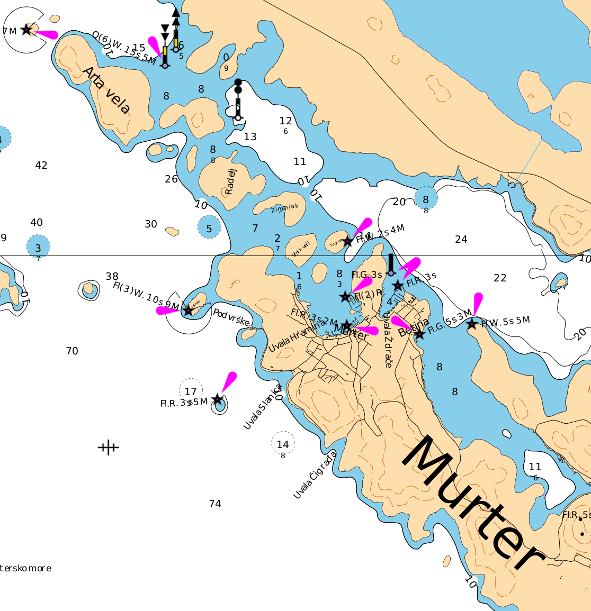
\includegraphics{inc/depth_cont}

   \caption{Directional filling.}\label{fig:dir}
\end{wrapfigure}

A typical application for the \emph{directional} fill mode on sea charts is the
rendering of depth contours, in particular if they are filled in shallow
inshore areas. \smrender{} takes care on the direction of the
polygons.\footnote{A few features exist in OSM as well of which the rendering
depends on the direction. Most importantly this is
\href{http://wiki.openstreetmap.org/wiki/Tag:natural=coastline}{natural=coastline}.
Other examples are
\href{http://wiki.openstreetmap.org/wiki/Tag:waterway=canal}{waterway=canal}
and
\href{http://wiki.openstreetmap.org/wiki/Tag:natural=cliff}{natural=cliff}.}
It always fills the portion which is \underline{left} of the way. Figure \ref{fig:dir}
shows an example. Shallow water with a depth less than 10 meters is rendered
blue, deeper areas are white (transparent). The white area northeast of the islet
Radelj is such a 20 meters area which is enclosed by a more shallow area and than
again by a deeper area on the west side of this chart detail.

Filling polygons using this mode works only if the polygons are edited correctly, i.e.
their direction is correct. Furthermore it is slightly slower than the regular fill mode.

\subsubsection{Placing Images} \label{sec:img}

Smrender allows to place images at the position of nodes or to fill areas using
an image as pattern.

\begin{verbatim}
   <definition>  := 'img:' [ <param> [ ';' <param> ... ]]
   <param>       := <name> '=' <value>
   <name>        := 'file' | 'angle' | 'scale' | 'mkarea' | 'anglekey'
\end{verbatim}

The parameter \optv{file} is mandatory and contains a path to a PNG file. If
\smrender{} was compiled with \textsf{librsvg2} (see Section \ref{sec:compile})
it supports SVG files as well. The image is placed with its center directly at
the position of the matching node without any modifications.

The parameter \optv{angle} specifies an angle between 0 and 360 degrees to which to image may be rotated before it is placed 
onto the map.

If \optv{angle} is set to ``\textsf{auto}'',
\smrender{} tries to find a rotation angle. This works as described
in Section \ref{sec:cap}. The rotation function does not take the image itself into account except its size.
The rotation test starts at direction East and rotates counterclockwise.
Obviously, this makes only sense if it is applied to asymmetric non-centered images, such as light flares.
On areas, ``\textsf{auto}'' has no effect.

The paramter \optv{anglekey} defines the name of the key of a tag which is used
to derive the angle of rotation during runtime. It is implemented in the same
way as it is for captions (see Section \ref{sec:cap}). Obviously, this does not work
together with \optv{angle=auto}. The latter is ignored if \optv{anglekey} is
set.

The parameter \optv{scale} allows to scale the image. A value greater than 1
will enlarge the image, if scale is less than 1 it will shrink the image.
\smrender{} allows to set a global scaling parameter which is applied to all
images, additionally. This is set with the command line parameter \optk{s}
(see Section \ref{sec:options}).

The parameter \optv{mkarea} is a boolean parameter. If set to \emph{yes}, the
auto-rotation function will add nodes and ways to the data which indicate the
level priority of the angles around the node. This is mainly intended for
debugging.


%bis hier
\subsection{Data Manipulation} \label{sec:manipulation}

\subsubsection{Adding Objects}

With this action you can add OSM objects as defined in the ruleset to the data.
You can use this to add specific OSM objects during during the stage of
rendering. Thus, you don't have to ``pollute'' your source data with
map-specific data before. Typically, those objects added are graphically
rendered by a subsequent rule. Currently, \smrender{} only OSM nodes are supported.
% FIXME in future this may be changed.

\begin{verbatim}
   <definition>  := 'add:' [ <param> [ ';' <param> ... ]]
   <param>       := <units> | <halign> | <valign> | <reference>
   <units>       := 'units' '=' <decval> [ <udef> ]
   <decval>      := a decimal number
   <halign>      := 'halign' '=' <hdef>
   <hdef>        := 'north' | 'south'
   <valign>      := 'valign' '=' <vdef>
   <vdef>        := 'east' | 'west'
   <reference>   := 'reference' '=' <ref>
   <ref>         := 'absolute' | 'relative'
\end{verbatim}

This function adds a node to the OSM data. All tags of the node are copied
except the \textsf{\_action\_} tag.  The position of the new node is derived
from its latitude and longitude. By default, the coordinates are treated as
absolute values referred to the geographic coordinate system. if
\optv{reference} is set to \optv{relative}, the coordinates are treated as
relative values to the center of the page. This can be influenced by the
parameters \optv{halign} and \optv{valign} in which case the origin is set to a
page border or page corner. The latitude and the longitude have to be set as
decimal number. With the parameter \optv{units} the unit of measurement can be
changed.  The default is \optv{degrees} but \optv{mm} (milimeters) or \optv{cm}
(centimeters) can be used as well. If \optv{relative} referencing used, positiv
values mean a shift to the right (eastern) and upwards (northern), negative
values shift to the left (western) and downwards (southern).

\paragraph{Example} The following example adds a node 7 centimeters to the
right and above of the lower left page corner.
\begin{verbatim}
<node lat="70" lon="70">
  <tag k="compass" v="yes"/>
  <tag k="name" v="2°05'E 2003 (5'E)"/>
  <tag k="bearing" v="2.0833"/>
  <tag
    k="_action_"
    v="add:reference=relative;halign=west;valign=south;units=mm"
   />
</node>
\end{verbatim}

\subsubsection{Adding Tags to Objects} \label{sec:addtag}

The action \textsf{set\_tags} allows to add an arbitrary number of OSM tags to an
object. The tags have to be defined through an object within the rules file.
This object may have no action tag. The template should have an id because
the action \textsf{set\_tags} needs to have a reference to it. To format simple
looks like the following.

\begin{verbatim}
   <action>    := 'set_tags:' <param>
   <param>     := <name> '=' <value>
   <name>      := 'id'
\end{verbatim}

Please note that the object type of the rule must be the same as the object
type of the template.

\subsubsection{Standard Shapes} \label{sec:shape}

\smrender{} is able to generate standard shapes like triangles, or circles using this action.
The formal definition looks like the following.

\begin{verbatim}
   <action>       := 'shape:' <param>
   <param>        := <name> '=' <value>
   <name>         := 'nodes' | 'style' | 'radius' |  'angle' |
                     'key' | 'weight' | 'phase' | 'start' |
                     'end' | 'subtype' | 'r2'
\end{verbatim}

This action internally generates an ellipse\footnote{Wikipedia: Ellipse, \url{http://en.wikipedia.org/wiki/Ellipse}.}
with the given \textsf{radius} (the semi-major axis $a$) and places a
number of \textsf{nodes} on its circumference.

Because OSM does
not support any kind of arcs natively, they are constructed using ways with a specific
number of nodes. The parameter \textsf{nodes} specifies this number of nodes.
Thus, for example, if \textsf{nodes} is set to 3, the result will be a
triangle.

The parameter \textsf{weight} is set to 1 by default if it is omitted. It is a multiplier
which is used to calculate the semi-minor axis $b = weight \times a$. Thus, if \textsf{weight = 1} a circle
is generated. The parameter \textsf{phase} shifts the points along the circumference in a counterclockwise order.
Thus, the following action creates a rectangle of the dimension
$4\times 1.2$ millimeters which is rotated by 20 degrees counterclockwise.
\begin{verbatim}
   <tag k='_action_'
        v='shape:nodes=4;radius=2;angle=20;weight=0.3;phase=45'/>
\end{verbatim}

One of the parameters \textsf{nodes} or \textsf{style} is mandatory. The latter
argument is a preset for a specific number of nodes. Currently the styles
\textsf{triangle} (= 3 nodes), \textsf{square} (= 4 nodes), and \textsf{circle}
(= maximum nodes) are supported.

The \textsf{radius} is given in millimeters and the optional parameter
\textsf{angle} may be used to rotate the shape at any degrees counterclockwise.
If \textsf{radius} is omitted 1 millimeter is used as a default value.

With \textsf{key} the shape may be rotated dependent on the value of a tag of a
node. \textsf{Key} defines the key of this tag.

This action does not render anything itself. It generates an according set of
new nodes which are connected together with a way. All these nodes and the way
get the tag \textsf{generator=smrender}.  The way additionally inherits all
tags of the original node which was matched by the rule set to invoke this
action. These tags can then be used to render the shape with a way rule. See
the following snippet as an example.

\begin{verbatim}
    <node version='-1'>
       <tag k='natural' v='peak'/>
       <tag k='_action_' v='shape:style=triangle;radius=.7'/>
    </node>
    <way>
       <tag k='natural' v='peak'/>
       <tag k='_action_' v='draw:color=#906030'/>
    </way>
\end{verbatim}


\subsubsection{Create Formatted Strings} \label{sec:strfmt}

This action is intended to create formatted strings out of a set of tags. It
works in a similar but yet more simple manner as \textsf{printf(3)} does. The
newly constructed string will be added as a new tag to the OSM object. This
tag may then be used to match on in subsequent rules.

\begin{verbatim}
   <action>       := 'strfmt:' <param>
   <param>        := <name> '=' <value>
   <name>         := 'addtag' | 'format' | 'key'
\end{verbatim}

\textsf{Strfmt()} has two mandatory arguments. The first one is \textsf{addtag}
which contains the name for the new tag which will be added to this object.
The second parameter is \textsf{format} which specifies a format string. It may
contain any characters and a set of format symbols. The format symbols are the
\textsf{\%} character followed by one of the following characters.

\begin{itemize}

   \item[\textsf{s}] The string of the value of the tag specified by the
      respective \textsf{key} is copied to the output string.

   \item[\textsf{f}] The string of the value of the tag specified by the
      respective \textsf{key} is interpreted as a floating point number and
      copied to the output string.

   \item[\textsf{d}] The string of the value of the tag specified by the
      respective \textsf{key} is interpreted as an integer number and copied to
      the output string.

   \item[\textsf{$\big[$n$\big]$r}] $n$ digits of the fractional part of a
      floating pointer number is copied to the output string as integer number.
      The number $n$ is optional. If it is omitted, 1 is assumed.

      Example: Let's assume that the original value is 3.1415, then the format
      specifier '\%r' would produce '1' as result, and if '\%2r' is specified
      the result would be '14'.

   \item[\textsf{\%}] The percent character is literally copied to the output
      string.

   \item[\textsf{v}] A semicolon is copied to the output string.

\end{itemize}

All regular characters are directly copied to the output string without conversion.
The action \emph{must} contain a \textsf{key} for each format symbol in the
format string. The keys are used exactly in the order as they appear in the
action line of ruleset.

\paragraph{Format String Example}

The following example shows how to create a new string for all peaks. It shows
the name of the peak and its elevation in parentheses. This string is then
rendered in the second rule.

\begin{verbatim}
<node>
   <tag k='natural' v='peak'/>
   <tag k='_action_' v='strfmt:format=%s (%s);
                  addtag=peak_string;key=name;key=ele'/>
</node>
<node>
   <tag k='peak_string' v=''/>
   <tag k='_action_' v='cap:font=serif;size=2;key=peak_string'/>
</node>
\end{verbatim}

\subsubsection{Concatenating Ways}

%  \item {\sffamily cat\_poly}

      This function closes open polygons. To have closed polygons is
      highly important because just such polygons can be filled with a
      background color.

      Polygons which are literally closed, such as the coastline or lakes are
      very often found as a set of open ways whose beginning and end share the
      same nodes. This is because different tags may be attached to different
      parts of the polygon. Furthermore, just partial data sets are used as
      input because typically just a small area out of the world's data is
      selected.\\

      \textsf{Cat\_poly} has three optional parameters: \textsf{ign\_incomplete},
      \textsf{no\_corner}, and \textsf{copy}. The first two can both be set to either 0 or 1. If these
      parameters are omitted, both are internally set to 0 by default.

      If \textsf{ign\_incomplete} is set to 1, \textsf{cat\_poly} will only
      close such polygons which are formed by a collection of ways where the
      end point of each way directly is the starting point of the next way.

      If \textsf{ign\_incomplete} is set to 0 (which is the default)
      \textsf{cat\_poly} will also close polygons which are still open even if
      all ways which have direct neighbors are connected by inserting
      artificial ways.  This is done by connecting the end of each way to the
      beginning of the next way in the clockwise order of the bearing from the
      center point of the image to the start/end nodes of the ways.

      Please note that the insertion of artificial ways only works properly if the ways have a
      specific direction. This is true at least for the ways which are tagged
      with \textsf{natural=coastline}.
      
      The parameter \textsf{copy} can occur multiple times and it is used to
      specify the keys of the tags of the ways which should be copied to the
      newly joined long way. If the values of these keys differ than
      \smrender{} takes just the first one. All others are ignored. This is
      because OSM defines that a tag can appear just excatly one time in an OSM
      object. \\

      If \textsf{cat\_poly} is applied in a way rule than \smrender{} tries to
      close all ways which match the criteria of the rule. The function finds all
      adjacent ways and closes them properly. The original data is not changed
      furthermore it creates and inserts new ways. Those new ways are tagged
      with all tags that where defined in the rule set plus the tag
      \textsf{generator=smrender} plus all tags which have been specified by
      the \textsf{copy} parameters.
      
      As already mentioned, a typical application for this function is to close
      the coastline which will be open in most cases. The coastline is always
      tagged with \textsf{natural=coastline}.

      If \textsf{cat\_poly} is applied to a relation then \smrender{} closes all
      ways of each relation separately. It creates a new closed way which will
      receive all tags of the relation, respectively. Additionally, it adds
      the tag \textsf{generator=smrender}. The tags of the way segments are join 
      to the new way if they are listed with the parameter \textsf{copy} as
      explained above.
      
      \textsf{Cat\_poly} applied to relations is useful for example in the
      Agean Sea, where all partial ways of an island are grouped together using
      relations. The tags of this relation contains global information about
      each island, such as its name or population. \\

      Please note that \textsf{cat\_poly()} may create ways with more the 2000
      nodes which violates the OSM standard definition.\footnote{See
         \url{http://wiki.openstreetmap.org/wiki/Way}.}. This may cause
         problems if an output file is created (e.g. with option \optk{w}) and
         used in other OSM applications. \smrender{} supports ways of up to
         $2^{31}$ nodes. It is assumed that most other OSM processing tools do
         not care about the artifical boundary of 2000.

      \subsubsection{Inherit Tags to Objects}
%   \item {\sffamily inherit\_tags} (\textsc{experimental})

\begin{verbatim}
   <action>    := 'inherit_tags:' [ <param> [ ';' <param> ] ]
   <param>     := <objdef> | <dirdef> | <force> | <keydef>
   <objdef>    := 'object' '=' <obj>
   <obj>       := 'node' | 'way' | 'relation'
   <dirdef>    := 'direction' '=' <dir>
   <dir>       := 'up' | 'down'
   <force>     := 'force' '=' <bool>
   <keydef>    := 'key' '=' <string>
   <string>    := any valid osm key string
\end{verbatim}


      This action copies tags from objects to their \emph{parent} or children objects depending on
      the value of \optv{direction}. A
      relation is considered as the parent of all of its members and a way is
      the parent of all of its nodes.

      There may be a list of one or more \optv{key} parameters and optionally
      the parameters \optv{object} and \optv{force}. The \optv{key}s specify
      which tags from the child (which is the object to which this rule is
      applied if \textsf{direction=up}) are copied to its parents -- and vice versa if \textsf{direction=down}.
      If \optv{object} is not defined, the
      tags are copied to all parents/children of any type. The parameter \optv{object}
      may be set to either \optv{way} or \optv{relation} in which only the
      parents of those types are taken into consideration.

      The parameter \optv{force} may be set to 0 (which is default) or 1. In
      the latter case \textsf{inherit\_tags} will overwrite tags in the parent
      if they do already exist.

         \subsubsection{Generating a Grid} %FIXME: not finished

         \begin{verbatim}
         grid()
         \end{verbatim}

      This action creates a grid exactly like the command line option \optk{g}
      but it provides more options.  It provides the parameters \optv{margin},
      \optv{tickswidth}, and \optv{subtickswith} to adjust the size of the axis
      rulers. Values are given in milimeters. Furthermore it provides the
      parameters \optv{grid}, \optv{ticks}, and \optv{subticks} which work
      exactly like the command line option (see Section \ref{sec:options}).
      Missing parameters are initialized with default values.


      \subsubsection{Create a Ruler}   %FIXME: not finished

      \begin{verbatim}
      ruler()
      \end{verbatim}
%   \item {\sffamily ruler}

      This function allows to generate a metric ruler. It is thought to be used
      for land maps.  It takes the arguments \optv{section} and \optv{count}.
      \optv{Section} is the length of one section of the ruler in kilometers.
      \optv{Count} sets the number of sections.

      \subsubsection{Text Translation}

\begin{verbatim}
   <action>    := 'translate:' [ <param> [ ';' <param> ] ]
   <param>     := <keydef> | <iddef> | <newtagdef>
   <keydef>    := 'key' '=' <keyval>
   <keyval>    := <string> | '/' <regex> '/'
   <iddef>     := 'id' '=' <objid>
   <newtagdef> := 'newtag' '=' <bool>
\end{verbatim}

   This function translates tag values. It can be used to e.g. translate text
   into different languages. The function looks up a given value in a
   translation table and replaces its value accordingly. If no entry is found
   in the translation table, no translation is performed.

   The keys whose values should be translated are given with the parameter
   \optv{key}. It can be specified several times to be applied to several tags
   of an object at once. The value of \optv{key} can be a simple string or a
   regular expression enclosed in \textsf{'/'}s.

   By default the values are replaced in-place. If the old value should be
   preserved, set the parameter \optv{newtag=1}. \smrender{} will then insert a
   new tag into the list of tags. Its value will be the translated value and
   the name of the key will be appended by the string '\textsf{:local}'.\\

   The translation table is defined in the ruleset as well like a template (see
   Section \ref{sec:addtag}). This is a rule node with an action. It has to have a node
   id because it is referred to by the \textsf{translate()}-rule. This
   translation object (the template) lists key-value-pairs being the key \textsf{k} the
   original value and the value \textsf{v} the one translated one.

   Have a look at Section \ref{sec:transexample} for a detailed example.


      \subsubsection{Special Data Manipulation Functions}

   \begin{itemize}

   \item {\sffamily clip}

      This function
      clips\footnote{\url{https://en.wikipedia.org/wiki/Clipping_\%28computer_graphics\%29}}
      to chart to a given border, i.e. it cuts of the rendered parts at the
      page border around to chart.

      The optional parameter to \textsf{clip()} is \optv{border} which takes 4
      decimal comma-delimited values. These are the 4 page border values
      (northern, eastern, southern, western) in millimeters, e.g.
      \optv{border=15,20,15,20}. If \optv{border} is omitted, \smrender{} clips
      to the default axis borders of the chart.

   \item {\sffamily dist\_median} (\textsc{experimental})

      This function calculates the median of the length of the edges of a way.
      It adds the tag \textsf{smrender:dist\_median=*}. The value of the tag
      contains the result of the calculation.

   \item {\sffamily ins\_eqdist} (\textsc{experimental})

      This function inserts nodes along a way with equal distances. The
      distance is given with the parameter \optv{distance} in any unit
      according to \ref{sec:units}. If no unit is specified, nautical miles is
      taken as default.
      The newly inserted nodes inherit all tags from the way and additionally
      the tags \textsf{generator=smrender}, and \textsf{distance=*}, and
      \textsf{bearing=*} are added. The latter two tags are set to the
      appropriate values. The bearing may be used by the function \textsf{shape}
      (see Section \ref{sec:shape}) to create appropriate rotated shapes.

   \item {\sffamily mask} (\textsc{experimental})
      
      This function allows to mask nodes if there is a dense cluster of nodes
      in some places on the chart which would make the result to look like just
      as a blur of color. Sometimes this is also called \emph{uncluttering}.

      The function has the parameter \optv{distance} which gives the distance
      of nodes in nautical miles which should be taken into account. This means
      that if there are more than one node within the given distance, just the
      most centered one is ``chosen''. All other nodes are tagged with
      \textsf{smrender:mask=yes}. This tag can then be matched on within the
      ruleset.

   \item {\sffamily poly\_area}

      This function calculates the area of closed polygons in nautical square miles. It
      adds the tag \textsf{smrender:area=*} to the way. The value of the tag contains
      the area.

   \item {\sffamily poly\_centroid}

      This function calculates the centroid of a closed polygon. It then adds a new node
      at this position. The node will inherit all tags of the polygon. Additionally,
      the tag \textsf{smrender:id:way=*} is added whose value is set to the ID of the
      way, respectively.
 
   \item {\sffamily poly\_len}

      This function calculates the length of a polygon in nautical miles. It
      adds the tag \textsf{smrender:length=*} to the way.

   \item {\sffamily set\_ccw} and {\sffamily set\_cw}

      Those functions set the direction of a closed way to either clockwise
      (``cw'') or counterclockwise (``ccw'').

   \item {\sffamily split}

      This action can be applied to nodes only. It splits all ways at the
      matching node into two parts.

   \item {\sffamily refine\_poly} (\textsc{deprecated})

      This function smooths the edges of polygons. It may take the function
      arguments \textsf{iteration} and \textsf{deviation}. The first defines
      the number of loops of the iterative refinement process (default = 3).
      The latter defines the maximum deviation of the original polyline in
      meters (default = 50). This avoids too high distortion of the polylines.

   \item {\sffamily reverse\_way}

      This function always reverses a way independent of its current direction.

   \item {\sffamily zeroway} (\textsc{experimental})

      Insert an artificial way of length zero at the matching node if the node
      is connecting two other ways. Such a way is a way with two nodes where
      both nodes have the same position.

         
\end{itemize}


\subsection{Special Purpose Functions} \label{sec:specfunc}

\subsubsection{Calling External Functions} \label{sec:func}

\smrender{} has the ability to call user-defined library functions. This feature provides
modularity and the flexibility to be extended on the fly without modifying the core.
Thus, \smrender{} can be used for nearly every kind of rule-based OSM file processing.
The library calls \textsf{dlopen(3)} and \textsf{dlsym(3)} are used to dynamically import those
functions.

The basic rule format is defined in the following.

\begin{verbatim}
   <definition>  := <function> '@' <library> [':' <param>
                    [ ';' <param> ... ]]
   <library>     := path/name of shared library
   <param>       := <name> '=' <value>
\end{verbatim}

\optv{Function} is the name of the function as it is exported by the shared
object \optv{library}. In particular, the exported symbol has to be named
\textsf{act\_}\optv{function}\textsf{\_main()}, i.e. it has to be prefixed by
``\textsf{act\_}'' and suffixed by ``\textsf{\_main}''.  If \optv{library} contains a \textsf{'/'}, the path is
resolved and the shared object loaded from that location.  Otherwise the
dynamic linker tries to find the library in the appropriate system
directories.\footnote{See \textsf{dlopen(3)} for details.}

Beside linking the function itself, \smrender{} tries to import the optional
functions \textsf{act\_}\optv{function}\textsf{\_ini()} and
\textsf{act\_}\optv{function}\textsf{\_fini()}.  These two functions may be
used for initialization and finalization of the main function.

The \optv{function} is called on each match of an OSM node. The initialization
function \textsf{act\_}\optv{function}\textsf{\_ini()} is called once directly
after the rules file was parsed before the first match. The finalization
function \textsf{act\_}\optv{function}\textsf{\_fini()} is called onced
directly after the last match.

The prototypes are defined as follows.

\flinput{inc/lib_protos.h}

\textsf{Act\_function\_main()} gets a pointer to the rule structure and the OSM
object which matched the rule. The object can be either a \emph{node},
a \emph{way}, or a \emph{relation}.

\flinput{inc/rule_decl.h}

The rule structure contains three pointers. The first one points to the OSM object of the rule
as defined in the ruleset. The \textsf{\_action\_} tag was removed by the rules parser.
The Second pointer is initialized to \textsf{NULL} by \smrender{} and is not touched any further.
It is thought to be used by the external functions to store arbitrary data.
Please note that all resources that have been claimed by the \textsf{\_ini()} function (such as heap memory)
have to be freed again by the finalization function \textsf{\_fini()}.
The third pointer of type \textsf{action\_t} contains all data which needs \smrender{}
for rule processing. Its contents should not be touched except you know what you are doing.
It is important that the action structure (\textsf{action\_t}) contains the parameters which 
may have been passed to the function through the ruleset. The function \textsf{get\_param()} shall
be used to retrieve their values. The first parameter is a constant string to the \optv{name}
of the parameter. The second parameter is a pointer to a \textsf{double} variable which will
receive the converted \optv{value} of the parameter. Of course this works only if the
parameter contains a decimal value. This pointer may be set to \textsf{NULL} if it is not used.
The third parameter to \textsf{get\_param()} is a pointer to the action structure of the rule.

\flinput{inc/obj_decl.h}

The type of object can be determined on examination of
\textsf{osm\_obj\_t.type}.  The variable may be set to either of
\textsf{OSM\_NODE}, \textsf{OSM\_WAY}, or \textsf{OSM\_REL}. The object can
then be type-casted to either a \textsf{osm\_node\_t}, a \textsf{osm\_way\_t},
or a \textsf{osm\_rel\_t}. All those OSM types are defined in
\textsf{osm\_inplace.h}.

The return value of the function controls the further behavior of \smrender{}
while applying this same rule. A return value of 0 means no error. \smrender{}
will call the function again at the next matching object. If the return value
is greater than 0 it behaves similar but outputs a message in the log file. The
message contains the return value. If a negative value is returned, \smrender{}
immediately stops applying this rule, calls the \textsf{\_fini()} function and
processes the next rule.

%The initialization function gets a \textsf{orule\_t} parameter which contains
%the rule definition.  The structure can be examined. The field
%\textsf{orule\_t.rule.type} is always set to \textsf{ACT\_FUNC}.
%\textsf{Orule\_t.rule.func.parm} is of type \textsf{char*} and points to
%\optv{param-str} which was set in the rules file. If no parameter was defined,
%it is set to \textsf{NULL}. Please note that if a \optv{param-str} should be
%passed to an internal function, \optv{libstr} \emph{must} be set to
%\textsf{``NULL''}.

Section \ref{sec:rfunc} explains how to write own (rendering) functions more in
detail.

\paragraph{Security Implications}

This feature basically allows any user to call arbitrary functions on the
system. Thus, \smrender{} should \textbf{never ever} be installed with file modes
SUID/GUID-root! This would be a potential security risk and might allow an
attacker with access to your system to compromise it.


\subsubsection{Output of OSM Data} \label{sec:output}

With the action \textsf{out} it is possible to create an OSM file which contains all the
objects which match.
\smrender{} will create one file for each action. This means that if the same
file name is used in several \textsf{out} actions, the latter will overwrite the earlier ones.
The action takes just one argument, the path to the file.

\begin{verbatim}
   <definition>  := 'out:' [ <param> [ ';' <param> ... ]]
   <param>       := <name> '=' <value>
   <name>        := 'file'
\end{verbatim}



\subsubsection{Executing Programs and Scripts} \label{sec:exec}

\smrender{} is able to run external 3rd-party programs and scripts. \smrender{}
communicates through \textsf{stdin}, \textsf{stdout}, and \textsf{stderr} of the program. The new
process is executed by the system call \textsf{execvp(3)} or
\textsf{execvpe(3)} if available.

\begin{verbatim}
   <action>       := 'exec:' <param>
   <param>        := <name> '=' <value>
   <name>         := 'cmd' | 'arg' | 'env' | 'osmhdr'
\end{verbatim}

The mandatory parameter \optv{cmd} defines the path to program. Optionally, one
or more arguments can be passed to the program by multiply specifying
\optv{arg}. The arguments are passed exactly in the same order as in the
action. 

The optional parameter \optv{env} can be used to set environmant variables. By
default, the program is executed with an empty environment.
\smrender{} provides an interactive interface to communicate with the process.

The parameter \optv{osmhdr} is an optional boolean argument and influences the
communication protocol as explained in the following Section.


\paragraph{The Communication Protocol}
is an interactive hybrid command line protocol. All information from
\smrender{} to the process is sent in XML format.  In turn for simplicity, the
process can use simple commands.

The communication is initiated by \smrender{} with an XML header and the
\emph{Smrender} header. The latter contains the version of the protocol and the
a string for the XML generator, similar to the OSM format.

\begin{verbatim}
<?xml version='1.0' encoding='UTF-8'?>
<smrender version='0.1' generator='smrender 3.0.r1535'>
\end{verbatim}

After this header all OSM objects which machted the rule are sent, one after
the other in OSM format version 0.6.  If the action has the parameter
\optv{osmhdr} set, each object is included in an OSM header as well.  The
following shows an example of an object including the OSM header, i.e.
\optv{osmhdr=yes}.
\begin{verbatim}
<osm version='0.6' generator='smrender'>
<node id="39273652" version="5" timestamp="2009-02-05T06:45:28Z"
   uid="67265" visible="true" lat="44.2128480" lon="15.4482687">
<tag k="created_by" v="Merkaartor 0.13"/>
</node>
</osm>
\end{verbatim}
If \optv{osmhdr} is omitted or set to \optv{no}, the first and the last line of
the above stanza are suppressed.  After each OSM object, \smrender{} waits for
commands of the process.  Every command will generate some output and finally
send a status code. The status code may be used by the process determine if a
command could be executed successfully.
\begin{verbatim}
<status code="200">OK</status>
\end{verbatim}

The following commands are currently implemented:

\begin{itemize}
   \item \textsf{.} [<code>]
      
      A single period on a line will provoke \smrender{} to send the next
      object which matches the rule. Optionally a numeric code between -128 and
      127 can be supplied. 0 is default (if omitted) and simply means success.
      \smrender{} appends the status code 200 to each object. If no more
      objects are available, status code 404 is sent. In that case \smrender{}
      waits for a last confirmation through a single period.
      
      A positiv number indicates an error.
      \smrender{} will stop further processing of objects of this rule. The
      process has the chance to finalize and has to commit this with a single
      period again. \smrender{} will close all streams and continue executing
      the next rule.

      If A negative number is returned, \smrender{} interpretes this as a fatal
      error. As a consequence it will imediately stop further processing.




   \item \textsf{get (node|way|relation) <id>}

      Additional OSM objects can be retrieved with this command.

\end{itemize}


\subsubsection{Special Control Functions} \label{sec:special}
%\subsection{Special Purpose Actions} \label{sec:special}
%Currently, \smrender{} provides the following functions.

\begin{itemize}
   \item {\sffamily diff} (\textsc{experimental})

      This function takes the argument \optv{file} (exactly like in the
      function \textsf{out}. See Section \ref{sec:output}.) and \optv{infile}.
      It compares the ids of all objects in \optv{infile} with all objects wich
      have been loaded by \smrender{} (option \optk{i}) and writes all objects
      which do not exist to \optv{file}.

   \item {\sffamily disable}

      This function disables the object to which it is applied. This is done by
      setting the attribute \textsf{visible=``false''}.  It is intended to be
      used to completely ignore certain objects during the rendering process.
      Please note that disabled objects cannot be re-enabled again because the
      rendering engine completely ignores invisible objects.

   \item {\sffamily enable\_rule} and {\sffamily disable\_rule}

      These actions take the mandatory argument \optv{id} which specifies the
      id of the rule to be enabled or disabled. They actually set the visibility to
      either true or false (see Section \ref{sec:rules}). Please note that enabling
      a rule which would have been rendered before this one according to its
      version and id is not executed it again.

   \item {\sffamily exit}

      This function forces \smrender{} to stop. No further rules will be
      processed and \smrender{} will create the output files according to the
      command line options. It behaves exactly like sending the \textsf{INT}
      signal (pressing \textsf{\^{}C}, see Section \ref{sec:sig}).

      This function is mainly intended for debugging rule sets.

   \item {\sffamily incomplete} (\textsc{experimental})

      This action can be applied to relations only.
      It takes the single parameter \optv{file} which specifies the
      name of the output file to which it will write the types and ids of all
      objects which are listed as members of the relation but are not found in
      the input data. This may be useful to download this objects to complete
      the input data if necessary.

      Please note that this currently may not work properly if you specify the
      same file name in several \textsf{incomplete}-rules.

   \item {\sffamily neighbortile} (\textsc{experimental})
      This is a special function which may be handy in the tile creation
      process.  It creates a directory named ``neighbor\_tiles'' and within
      this a tile directory tree (\textsf{zoom/x/y.conf}).  The files created
      within this will contain several variables suitable for being sourced in
      a shell script. The variables in the files specifies the bounding boxes
      of the tiles in zoom level 10. This function will be improved in future
      and the file format may change.


   \item {\sffamily sub} (\textsc{experimental})
      Call a set of sub-rules.

\end{itemize}


\section{Signals} \label{sec:sig}

\smrender{} installs two signal handlers, one for \textsf{SIGUSR1} and one
for \textsf{SIGINT}.
%Both signals are intended to be called during the process of reading OSM input
%data.

If \smrender{} receives a \textsf{USR1} signal during the process of reading
OSM input data, it outputs some statistics about the current position of
reading and data throughput. It may be used as progress indicator if huge files
are used as input.  If \smrender{} receives a \textsf{INT} signal (which is typically generated by pressing \textsf{\^{}C}) during
rendering, it immediately aborts rendering of further objects and saves the image
in its current state and exits normally. If \textsf{SIGINT} is caught twice, \smrender{}
exits immediately.


\section{Extensions}

As explained in Section \ref{sec:func}, \smrender{} is able to call functions
of shared objects through dynamic linking at runtime. Thus it is very easy to
extend the core functionality of \smrender{}.  Currently, it comes with one
additional library which is \textsf{libsmfilter}.


\subsection{Libsmfilter and Smfilter} \label{sec:smfilter}

\textsf{Smfilter}\footnote{See \url{http://www.abenteuerland.at/smfilter/}} is
a preprocessor for Osmarender.  It adds some sea chart specific virtual nodes
and ways to simplify the rendering process.  The functionality of
\textsf{smfilter} is now integrated into \smrender{} with
\textsf{libsmfilter}. As a result, \textsf{smfilter} is no longer supported.
\textsf{Libsmfilter} exports four functions: \textsf{vsector()}, \textsf{pchar()}, \textsf{compass()}, 
and \textsf{sounding()}.
The first is the replacement for \textsf{smfilter}, the next is a new function which
generates combined strings for light descriptions, the third creates a magnetic
variation compass, and the last generates nodes and ways for
depth soundings as used in sea charts.

All functions belong to the category \emph{data manipulation} (see Section
\ref{sec:manipulation}), which add OSM objects to the data. Thus, graphical
rendering rules (see Section \ref{sec:rendergfx}) are necessary to display
those objects on the page.

\subsubsection{Generating Light Sectors with vsector()}

This function is a full replacement for \textsf{smfilter}.
\textsf{Smfilter} took several options\footnote{See
\url{http://www.abenteuerland.at/smfilter/smfilter.html}} to adjust the
rendering behavior. These are the options \optk{a}, \optk{b}, \optk{d}, and
\optk{r} in particular.  \textsf{Libsmfilter} now takes exactly the same
parameters since it is just a port.  The parameters must be fed to it within
the rules file. This was commonly described in Section \ref{sec:func}.
In detail the format looks like the following.

\begin{verbatim}
   <param-str>   := <a-v-pair>[';' <a-v-pair>[';' ...]]
   <a-v-pair>    := <attribute> '=' <value>
   <attribute>   := 'a' | 'b' | 'd' | 'r' | 'f'
   <value>       := decimal number
\end{verbatim}

\begin{itemize}
   \item[\textbf{a}]

    This sets the maximum distance of arc nodes. Basically, the distance is
    scaled with the radius; the smaller the radius the smaller the distance and
    vice versa. With large radii the distance of nodes is limited to dist. The
    value is given in nautical miles. 

 \item[\textbf{b}]

    Leading and directional lights are rendered with a bearing line and a small
    arc at its end. deg sets the angle of this arc to one side which means it
    is drawn def degrees clockwise and def degress counterclockwise from the
    bearing line. 

 \item[\textbf{d}]

    This defines the arc divisor which is used to determine the distance of the
    arc nodes. Thus, the node distance equals the radius divided by div. (see
    also option -a). 

 \item[\textbf{r}]

    A light may not have any radius specified since the tag is optional. In
    such cases smfilter picks radius as default value. 

 \item[\textbf{f}]

    This is a scaling factor for all radii. In particular, this can be useful
    for charts in very large scales. The default value is 1.

\end{itemize}

This is an example for calling \textsf{vsector()} from the rule set.

%\begin{lstlisting}[language=XML,basicstyle=\footnotesize]
\begin{verbatim}
<node>
   <tag k='seamark:type' v=''/>
   <tag 
      k='_action_'
      v='vsector@libsmfilter.so:a=0.05;d=20;r=0.5'
   />
</node>
\end{verbatim}
%\end{lstlisting}

A full description of the output produced by \textsf{vsector()} is found in the
\textsf{smfilter(1)} man
page\footnote{\url{http://www.abenteuerland.at/smfilter/smfilter.html}} and in the
OSM wiki.\footnote{\url{http://wiki.openstreetmap.org/wiki/OpenSeaMap/smfilter}}

\subsubsection{Compatibility to Smfilter}

The function \textsf{vsector()} does exactly the same as the original \textsf{smfilter} tool.
Thus, they are considered to be nearly 100\% compatible.
The functionality is exactly the same but the file structure will still be different because
\smrender{} processes the OSM file in a different way than \textsf{smfilter}.

The following shows two exchangable command lines, the first for \textsf{smfilter} and
the second for \smrender{}.\\

\rbox{smfilter -a 0.05 -d 20 -r 0.5 < in.osm > out.osm}

\rbox{smrender -i in.osm -o /dev/null -M -G -w out.osm}\\

The following rules file has to be used in conjunction with \smrender{} to be a 
replacement for \textsf{smfilter}. Of course, the file may be extended with 
other rendering rules.

\begin{verbatim}
<?xml version='1.0' encoding='UTF-8'?>
<osm version='0.6'>
   <node>
      <tag k='seamark:type' v=''/>
      <tag k='_action_'
           v='func:vsector@./libsmfilter.so?a=0.05,d=20,r=0.5'/>
   </node>
</osm>
\end{verbatim}


\subsubsection{Generating Light Description Strings}

\textsf{Pchar()} generates a string which contains the characteristics of the
light as it is used in official sea charts and the \emph{List of Lights}. See
Section P and P.16 in particular if the \emph{Chart No.
1}.\footnote{\url{http://www.nauticalcharts.noaa.gov/mcd/chart1/ChartNo1.pdf}}

The function analyzes the tags of an object. If it contains valid
\emph{OpenSeamap} tags\footnote{See
\url{http://wiki.openstreetmap.org/wiki/OpenSeaMap/Lights_Data_Model}.} it
generates the light string and adds the new OSM tag
\textsf{seamark:ligh\_character=*} to the object. The value of the tag contains
the string which may be rendered by a subsequent rule.

Since the description of lights varies in different languages, \smrender{}
supports the optional parameter \optv{lang} which may be set to either
\textsf{'de'} for German or \textsf{'hr'} for Croatian language. If the
parameter is omitted it defaults to English. The following table shows language
examples according to \emph{INT-1, IP 51}:\\

\begin{tabular}{l|l}
   English & \textsf{Fl.10s 40m 27M} \\
   German & \textsf{Blz.10s 40m 27sm} \\
   Croation & \textsf{B Bl 10s 40m 27M} \\
\end{tabular}


\subsubsection{Generating a Magnetic Variation Compass}

This function creates a magnetic variation compass as usual on sea charts. This
is a north-up compass with with crosslines rotated by the variation as shown in Fig. \ref{fig:compass}.
As most other functions,
it will not directly create graphics output but OSM nodes and ways with specific tags.
Those can then be graphically rendered by using one of \smrender's rendering
primitives (s. Section \ref{sec:cap} and \ref{sec:draw}).

\begin{verbatim}
   <definition>  := 'compass@libsmfilter.so:' [ <param> [ ';'
                                                <param> ... ]]
   <param>       := <name> '=' <value>
   <name>        := 'variation' | 'radius' | 'ticks'
\end{verbatim}

\begin{wrapfigure}{r}{45mm}
   \centering
   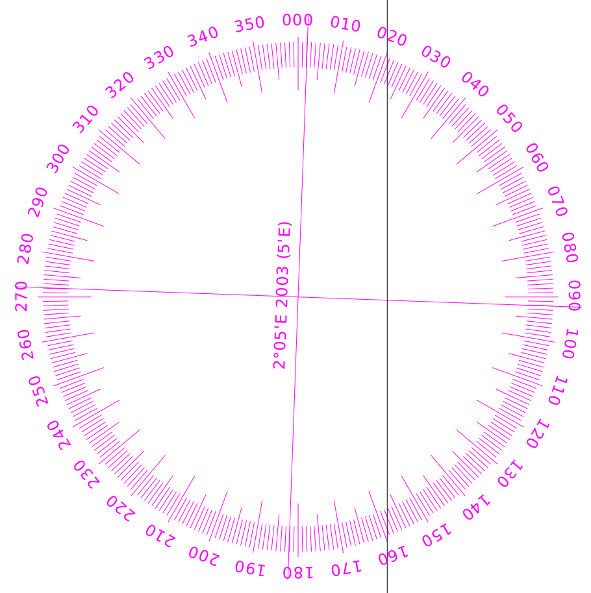
\includegraphics[width=42mm]{inc/compass}

   \caption{Magnetic variation.}\label{fig:compass}
\end{wrapfigure}
The parameter \optv{radius} is mandatory and defines the outer radius of the
compass. It is given as degrees on a Meridian.\footnote{This is subject to being
improved in future releases.} %FIXME

The parameter \optv{variation} sets the variation, i.e. the amount of degress
to which the crosslines will be rotated. It is set in degrees. A positive value
denotes eastern variations.

The parameter \optv{ticks} defines the number of ticks on the circle. The default
value is 360.\\

All newly created nodes and ways are tagged with \textsf{smrender:compass=*}
containig the bearing of the way in degrees. Every tenth outer node is
additionally tagged with \textsf{smrender:compass:description=*} containing the
bearing in degrees as well but with a leading zero as usual for the description
of degrees on a sea chart.

See Section \ref{sec:compasssample} for a complete example.


\subsubsection{Generating Circles around Depth Soundings}

\textsf{Libsmfilter} provides the function \textsf{sounding()} which generates
small circles around depth soundings.

It generates symbols such as I.4 of Chart No. 1 and circles with a dashed line used for approximate
depths (I.31).

Tags use for it is \textsf{seamark:sounding=*} containing the depth in meters,
and optional \textsf{seamark:sounding: quality = \{approx $\Big|$ reported\_unconfirmed\}}.
See \href{http://www.cypherpunk.at/2012/03/11/rendering-depths-with-smrender/}{``Rendering Depths with \smrender''}\footnote{\url{http://www.cypherpunk.at/2012/03/11/rendering-depths-with-smrender/}} for 
more details.

\section{Usage Examples} \label{sec:samples}

There is a very simple example for your first rendered map. Before, download,
compile, and install \smrender{} as explained in Section \ref{sec:compile}.

Create a working directory somewhere.
From the \smrender{} download URL\footnote{\url{http://www.abenteuerland.at/smrender/download/}} get the seamap icons package (\textsf{icons.tbz2}) and
extract it.

\begin{verbatim}
tar xvfj icons.tbz2
\end{verbatim}

Now we have to get some OSM data. We just use the Overpass API\footnote{\url{http://wiki.openstreetmap.org/wiki/Overpass_API}.} to get a small window.

\begin{verbatim}
wget -O cr.osm \
   'http://www.overpass-api.de/api/xapi?map?bbox=15,43.7,15.4,44'
\end{verbatim}

Now we can start \smrender{} by using the rule set \textsf{rules.osm} which comes
with the \smrender{} package. Copy it to your working directory. By default it is installed into \textsf{/usr/local/share/smrender}.

\subsection{Generating a PDF} \label{sec:genpdf}

PDF files are the best choice if you intend to print something.
The following command line renders the OSM file \textsf{cr.osm}
to the output image \textsf{cr.png} having the dimension of an A4 landscape page. 43° N 52.8' 
15° E 12.8' are the center coordinates and the scale is chosen to be 1:100000 which is typical for sea charts.

\begin{verbatim}
smrender -i cr.osm -o cr.png -P A4 -l 43N52.8:15E12.8:100000
\end{verbatim}

The result is the PNG image \textsf{cr.png}. You may look at it using your
favorite image viewer. To get a correct non-distorted print-out it usually is a
good idea to use the PDF format instead. If you try to print the image with a
graphics program it most probably will be rescaled to fit the print margins.
This will usually not happen if you print a PDF which has valid paper
dimensions.
To create a PDF file use the option \optk{O} instead.

\begin{verbatim}
smrender -i cr.osm -O cr.pdf -P A4 -l 43N52.8:15E12.8:100000
\end{verbatim}


\subsection{Generating a KAP File} \label{sec:genkap}

KAP files are used by many applications that deal with marine navigation (e.g.
\emph{OpenCPN}, \url{http://opencpn.org/}) or GPS chart plotters or smart
phones (e.g. \emph{Marine Navigator} for Android,
\url{https://play.google.com/store/apps/details?id=de.kemiro.marinenavigator}).
Very often those files are also referred to as BSB files or also RNC files.

The following command generates a KAP file. It assumes
that you have an input OSM file \textsf{cr.osm}.  See the beginning of this
Section (Section \ref{sec:samples}) on how to retrieve it. The density is
reduced to 200 dpi (option \optk{d}) to save resources of your smart phone or
chart plotter.  Option \optk{G} disables the grid since most applications are
able to generate a grid on their own. The KAP file is saved to \textsf{cr.kap}.
The option \optk{s} \optv{1} disables antialiasing. This also reduces resource
usage because it limits the color space.  Many plotting applications may have
their built-in antialiasing.

\begin{verbatim}
smrender -i cr.osm -d 200 -G -k cr.kap -s 1 43N52.8:15E12.8:100000
\end{verbatim}

Please note that a PNG file and a KAP file may be generated at the same time by simply adding option \optk{o}.
The file \textsf{cr.kap} can be used by your favorite application. If you use
e.g. \emph{Marine Navigator} on Android you have to copy the file to a folder
named \textsf{BSB\_ROOT} in the root directory of your SD card.

\section{Ruleset Examples} \label{sec:rulesamples}

\subsection{Creating a Magnetic Variation Compass} \label{sec:compasssample}

{\small
\begin{verbatim}
<node lat="70" lon="70" version="-10">
   <tag k="compass" v="yes"/>
   <tag k="name" v="2°05'E 2003 (5'E)"/>
   <tag k="bearing" v="2.0833"/>
   <tag
    k="_action_" 
    v="add:reference=relative;halign=west;valign=south;units=mm"
    />
</node>
<node version="-10">
   <tag k="compass" v="yes"/>
   <tag
    k="_action_" 
    v="compass@libsmfilter.so:radius=0.03;variation=2.0833"
    />
</node>
<node>
   <tag k="compass" v="yes"/>
   <tag
    k='_action_'
    v='cap:font=sans-serif;color=magenta;size=2;key=name;
           anglekey=bearing;angle=-270;valign=north'
    />
</node>
<node>
   <tag k="smrender:compass:description" v=""/>
   <tag
    k='_action_'
    v='cap:font=sans-serif;color=magenta;size=2;
           key=smrender:compass:description;
           anglekey=smrender:compass;angle=0;valign=north'
    />
</node>
<way>
   <tag k="smrender:compass" v=""/>
   <tag k="_action_" v="draw:bcolor=magenta;width=0.2"/>
</way>
\end{verbatim}
}

\subsection{Translation Example} \label{sec:transexample}

   The following paragraphs demonstrate a translation of tags.
   First we need a translation table. The following shows a translation table
   for translating colors from English to German.

\begin{verbatim}
<node id='1000'>
   <tag k='red' v='rot'/>
   <tag k='green' v='grün'/>
   <tag k='blue' v='blau'/>
   <tag k='yellow' v='gelb'/>
</node>
\end{verbatim}

Now we want to apply the translation to seamark nodes which have English names
for the color of the lights. The name of these tags are either
\textsf{'seamark:light:colour=*'} or \textsf{'seamark:light:}\textsf{<N>:}\textsf{co\-lour=*'}
where \textsf{<N>} is any integer greater than 0. A node can have multiple such
tags. The rule should then look like this:
\begin{verbatim}
<node>
   <tag k='/seamark:light:.*colour/' v=''/>
   <tag
      k='_action_'
      v='translate:id=1000;key=/seamark:light:.*colour/;newtag=1'
   />
</node>
\end{verbatim}

Let's look at the following node which could be within the input data.
\begin{verbatim}
<node id='12345678' version='1' lat='47.1234' lon='10.2323'>
   <tag k='name' v='Red-White-Lighthouse'/>
   <tag k='seamark:light:1:colour' v='yellow'/>
   <tag k='seamark:light:2:colour' v='red'/>
   <tag k='seamark:type' v='beacon_lateral'/>
</node>
\end{verbatim}

\smrender{} will modify it according to the translation rule of above like follows.

\begin{verbatim}
<node id='12345678' version='1' lat='47.1234' lon='10.2323'>
   <tag k='name' v='Red-White-Lighthouse'/>
   <tag k='seamark:light:1:colour' v='yellow'/>
   <tag k='seamark:light:1:colour:local' v='gelb'/>
   <tag k='seamark:light:2:colour' v='red'/>
   <tag k='seamark:light:2:colour:local' v='rot'/>
   <tag k='seamark:type' v='beacon_lateral'/>
</node>
\end{verbatim}


\section{Files}

The \smrender{} package contains all source C files and headers. A
\textsf{configure} script is provided to create appropriate \textsf{Makefile}s
and build \smrender{} (see Section \ref{sec:compile}). It contains all sources
for the \textsf{smfilter} library (see Section \ref{sec:smfilter}) in the
directory \textsf{libsmfilter/} and a skeleton libary in the directory
\textsf{libskel/} which may be used as a starting point for own functions (see
Section \ref{sec:rfunc}). Due to an internal code reorganization many general
purpose functions are moved to the separate library \textsf{libsmrender}. All
respective sources are found in the directory \textsf{libsmrender/}.

The package contains futhermore different rule sets which may also be used as a basis for
own rule sets. The main ruleset is found in the directory \textsf{rules\_100000} which is actively maintained.
Older files are \textsf{rules.osm}, \textsf{rulesbig.osm}, and \textsf{rules\_land.osm} which are still
provided with \smrender.

\section{Bugs and Caveats}

\smrender{} does not validate the well-formedness of the OSM files. Thus, you may get unexpected rendering results if the file
format is incorrect.

For more information please look at the project homepage at \url{http://www.abenteuerland.at/smrender/}.

\section{Author}

\smrender{} is written by Bernhard R. Fischer, \url{mailto:bf@abenteuerland.at}. The idea of the project was born
in summer of 2010.  The actual development started in October of 2011.

\section{Copyright}

{\sffamily
       Copyright 2011-2015 Bernhard R. Fischer.\\

       This file is part of \smrender{}.\\

       \smrender{} is free software: you can redistribute it and/or modify it
under the terms of the GNU General  Public License as published by the Free
Software Foundation, version 3 of the License.\\

       \smrender{} is distributed in the hope that it will be useful, but WITHOUT
ANY WARRANTY; without even the implied warranty of MERCHANTABILITY or FITNESS
FOR A PARTICULAR PURPOSE.  See the GNU General Public License for  more
details.\\

       You  should  have  received  a  copy  of  the  GNU  General  Public
License  along with \smrender{}. If not, see $<$\url{http://www.gnu.org/licenses/}$>$.
}



%\section{Application}
%
%\subsection{Filter Mode} \label{sec:filter}
%

\clearpage

\appendix

\section{Compiling and Installing} \label{sec:compile}

\smrender{} should be simple to compile. It depends on
\textsf{libcairo}\footnote{\url{http://www.cairographics.org/}} and optionally
on \textsf{fontconfig} and \textsf{librsvg2}. Although they are not mandatory
it is still suggested to use those packages. With \textsf{fontconfig} you can
specify simple font faces such as e.g. \textsf{sans-serif} or
\textsf{DejaVuSans} and the package will handle the path resolution to the
necessary font files. You can still use fonts even without \textsf{fontconfig}
but you then have to specify the full paths for the font files in the
\textsf{cap()} rules (see Section \ref{sec:cap}) such as e.g.
\textsf{/usr/share/fonts/truetype/dejavu/DejaVuSans.ttf}. The package
\textsf{librsvg2} is used to read SVG images in your ruleset, otherwise it
supports just PNG images (see Section \ref{sec:img}).

If none of those packages is not installed, \smrender{} will still compile and
it can be used for OSM data processing but not for rendering charts (graphics
output).

Download the most recent \smrender{} package from its main URL.\footnote{\url{http://www.abenteuerland.at/download/smrender/}}
The packages includes the source code, some sea chart rulesets and a few
ruleset examples, and a skelleton library (\textsf{libskel}) to show how to
implement an own library with extension functions. It further includes
\textsf{libsmfilter} for rendering special sea chart features (see Section
\ref{sec:smfilter}), and a complete set of SVG icons for sea charts (buoys, beacons,\dots).\\

Extract the package with \textsf{xzcat | tar xv smrender-4.0.r$xxxx$.xz}. Change into the newly extracted
directory.
Then run the configure script \textsf{./configure}, then build it with \textsf{make}. It should compile fine. Finally, there is the executable \textsf{smrender} and
the \textsf{libsmfilter.so}. The latter is not mandatory for running \smrender{} since it
may just be loaded dynamically by the rule set (see Section \ref{sec:smfilter}). Those files
may be installed into the appropriate directories on your system with \textsf{sudo make install}.\footnote{Root privileges are required to install.}

\smrender{} is known to compile with \textsf{gcc 4.x} on Debian Linux (Lenny,
Squeeze, and Wheezy), FreeBSD version 8.x - 10.x, OpenBSD 5.x, and Mac OSX. It should compile on most Unixoid
plattforms without further troubles, maybe even on Windows with Cygwin.


\section{Writing Own Rendering Functions} \label{sec:rfunc}

The \smrender{} package includes a skeleton library in the directory \textsf{libskel/}.
It implements the library constructor and destructor, and the actual rule function together
with its initialization and de-initialization functions.

The directory contains also a \textsf{Makefile} which shows how to compile the library.\\

\smrender{} exports several functions which may be called by the library. The following list
shows the most imported ones. The prototypes are defined in \textsf{smrender.h}, \textsf{smlog.h}, or
\textsf{osm\_inplace.h}.


\flinput{inc/export_funcs.h}




\section{FAQ}

This section covers some questions and answer which might arise.

\subsection{Why is Smrender not written in C++?}

On closer examination, the software architecture suggests an object-oriented
programming language such as C++ but \smrender{} is written in C. The short
answer is that C is always my first choice and the code was already too mature
to switch to C++ without a high effort. The long answer is that \smrender{} is
able to dynamically link libraries at runtime. Interfacing from C++ to a
library written in C (currently) seems to be difficult (although not
impossible).

But I still have in mind to rewrite \smrender{} in C++ when time comes.

\subsection{Is it possible to create other maps, such as road maps?}

Yes of course! The appearance of the map solely depends on the ruleset. A very simple
first ``land'' ruleset is found in the rules directory.
The
only thing which is fixed is that \smrender{} uses a Mercartor
projection which typically is not used for ``land maps''.

\section{ToDo}

Software is never finished and I have a long list of ideas in mind which I could implement.
\begin{itemize}
%   \item The simple \textsf{Makefile} will be replaced by a configuration by the GNU \textsf{autotools}.
%   \item The GD library may be replaced by the more powerful \emph{Cairo} library.\footnote{\url{http://cairographics.org/}}
%   \item The action format will be replaced by a more flexible CSS-style format.
   \item Rendering of rotated (not North-up) maps.
   \item Dynamic rules; these are rules which are generated during the rendering itself and are applied
      subsequently.
   \item Automatic font size for bays and capes (similar to the font size selection algorithm of polygons/islands).
   \item \smrender{} as an OSM database server with a Websockets interface (development started with version 4.0).
\end{itemize}

%\phantomsection
%\addcontentsline{toc}{chapter}{Quellenverzeichnis}

%\section{Rulesfile}
%\label{sec:rulesfile}
%\lstinputlisting{rules.osm}

%\vfill

%
\includegraphics[scale=0.5]{schneggendier_600dpi_16mm}

\end{document}

